\documentclass[a4paper]{scrreprt}
\setcounter{tocdepth}{3}
\setcounter{secnumdepth}{3}

\usepackage[german]{babel}
\usepackage[utf8]{inputenc}
\usepackage[T1]{fontenc}
\usepackage{ae}
\usepackage{graphicx}
\usepackage{tabu}

\begin{document}
\title{Entwurf}
\author{Fangzhou Bian, Kathrin Blum, Matthias Bruns, \\Leonhard Duda, Tan Grumser, Yuguang Lin}
\maketitle
%\Footnote für Fußnoten
% Platzierung des Inhaltsverzeichnisses
\tableofcontents



\chapter{Einleitung}
Dies ist das Entwurfsdokument für die Applikation \dq MensaMeet\dq.  Es ist das Artefakt der Entwurfsphase, die direkt an die Definitionsphase anschließt, aus welcher das Pflichtenheft hervorging.
In den folgenden Kapitel wird auf die Systemarchitektur (\dq Grobentwurf\dq) eingegangen. Es folgt die Erläutereung der Systemkomponenten, sowie der verwendeten Frameworks und Schnittstellen. Im Kapitel \dq Feinentwurf\dq werden die Klassendiagramme der einzelnen Pakete im Detail vorgestellt und das verwendete HTTP Protokoll aufgeührt. Unter \dq Datenstrukturen\dq findet sich die Strukturiereung unserer Datenbank wieder. 
Im Abschnitt \dq dynamische Modelle\dq werden an Hand von Sequenzdiagrammen einige Abläufe von MensaMeet anschaulich dargestellt.
Schließlich Begründen wir in Kapitel 6 die Änderungen gegenüber dem Pflichtenheft.
Auf den letzten Seiten dieses Dokuments findet sich ein Glossar und ein vollständiges Klassendiagramm für die gesamte Applikation MensaMeet.



\chapter{Grobentwurf}
\section{Systemarchitektur}
Die App MensaMeet wird als Client-Server Anwendung umgesetzt. Clients fordern Dienste an, welche vom zentralen Server bereitgestellt werden. Dazu erhält jeder User der sich registriert ein eindeutiges UserToken, das auf seinem Endgerät gespeichert wird. Der Server verwaltet eine Datenbank, in welcher die Mensadaten und User- und Gruppeninformationen gehalten werden. 
Die Client-Seite der Anwendung wird mithilfe der MVVM (Model-View-Viewmodel) Architekur umgesetzt.
Die Server-Seite mithilfe der MVC (Model-View-Control) Architektur.
\section{Systemkomponenten}

\subsection{Client}
Die Client Seite bedient sich der MVVM Architektur. Die View dient zum anzeigen von Daten, sie beinhaltet alle grafischen Elemente, stellt also die GUI dar. Im Model werden die Daten gehalten und Funktionen zur Manipulation der Daten bereitgestellt.
Das Viewmodel enthält die Darstellungslogik für die View und kapselt sie von der Anwendungslogik, die sich im Model befindet, ab.
View und Viewmodel sind durch Databinding nur lose gekoppelt, dadurch kann die View problemlos ausgetauscht werden bzw. können mehrere verscheidene Views (z.b. angepasst an Tablet, Desktop,...) zum selben Viewmodel existieren.
Das Datainding kann als bidirektionaler Beobachter verstanden werden: View und Viewmodel kennen die interne Struktur voneinander nicht, aber Benachrichtigen einander, wenn es Änderungen gibt. Diese lose Kopplung durch Databinding verbessert die Testbarkeit, da so View und Viewmodel unabhängig voneiander getestet werden können.

\subsection{Server}
Für die Server Seite wird die MVC Architektur verwendet.
Das Model ist für die Datenhaltung zuständig und beinhaltet/verwaltet eine Datenbank.  In unserem Fall wird die relationale Datenbank MySQL verwendet. Als Kommunikationsschnittstelle zwischen der Datenbank und den Controllern des Servers wird JPA (Java Persistance API) mit Hibernate genutzt.
View ist durch eine Schnittstelle gegeben, über die der Server Anfragen des Client empfängt und an den Controller delegiert. Der Controller führt diese Anfragen durch, indem er angefordere Daten aus dem Model holt oder neue Daten einfügt bzw Daten anpasst.

\subsection{Frameworks und Interfaces}
\subsection*{JPA und Hibernate}

Objektrelationales Mapping (ORM) ist eine Technik der Softwareentwicklung, mit der ein (in objektorientierten Programmiersprache geschriebenes) Programm seine Objekte in einer relationalen Datenbank ablegen kann. Dem Programm wird dazu eine objektorientierte Sicht auf die Tabellen und Beziehungen im Datenbankmangemantsystem (DBSM) geboten. \\  \\ Wir benutzen das Java Persistence Application Programming Interface (JPA). \\ JPA ist eine API für Datenbankzugriffe und objektrelationales Mapping und muss durch einen sogenannten JPA Provider implemetiert werden. Wir implementieren JPA mithilfe des Frameworks Hibernate.\\ \\ Die Vorteile von Hibernate liegen vor allem in der Abstraktion der verwendeten Datenbank. Hibernate kann normale Objekte (Plain Old Java Object, POJO) in relationalen Datenbanken speichern und aus den Datensätzen der Datenbank wiederum Objekte erzeugen. Daher müssen keine SQL-Statments geschrieben werden, was die Implemenntierung erleichtert und die Entwickling der Anwendung effizienter macht. \\  Außerdem ist Hibernate, durch die Abstraktion, kompatibel mit verschiedenen Datenbanken, sodass die verwendete Datenbank (in unserem Fall MySQL) jederzeit leicht gegen eine andere relationale Datenbank ausgetauscht werden kann.

\subsection*{Spring}
\subsection*{Firebase}

\chapter{Feinentwurf}
\section{Klassen des Clients}
\subsection{Klassendiagramm}
\subsubsection{package.edu.kit.mensameet.model}

\newpage

\subsubsection{package.edu.kit.mensameet.view}
\begin{center}
	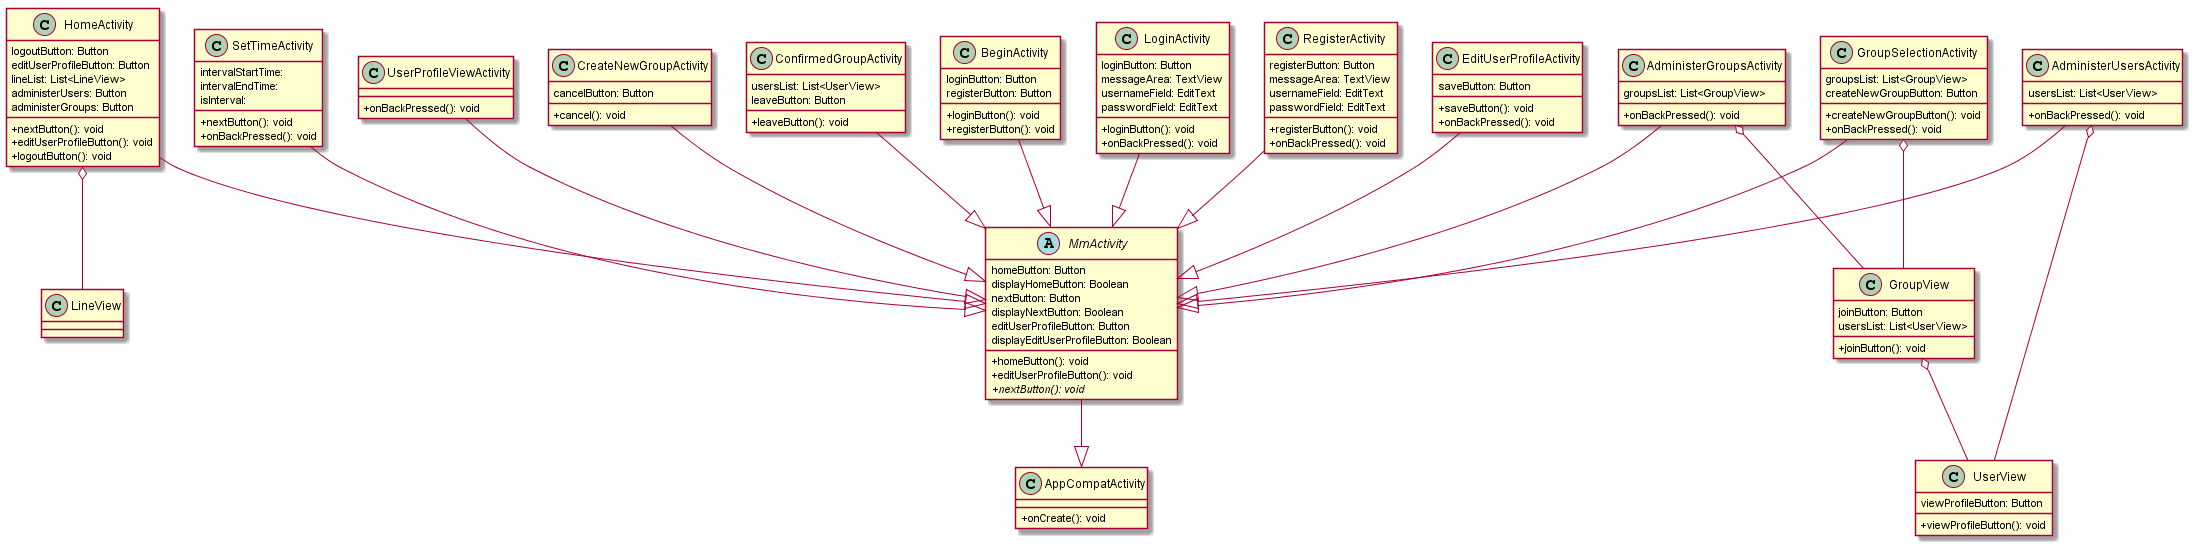
\includegraphics[width=0.99\textwidth]{GUI/frontend_view.png}
\end{center}


\newpage
\subsubsection{package.edu.kit.mensameet.viewmodel}
\begin{center}
	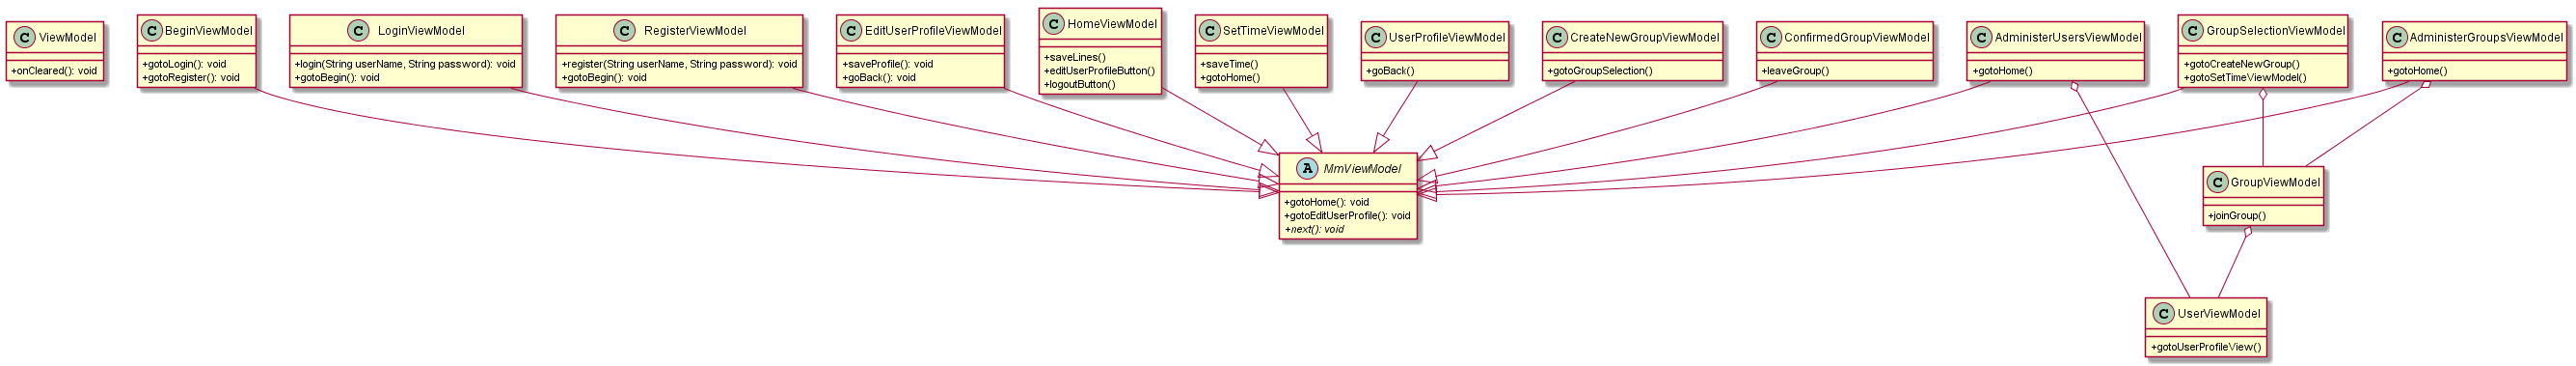
\includegraphics[width=0.99\textwidth]{GUI/frontend_viewmodel.png}
\end{center}

\section{Klassen des Server}
\subsection{Klassendiagramm}

\subsection{package.edu.kit.mensameet.model}
%Javadocs für Model%
\subsubsection{Class Group}
Die folgenden Klassen enthalten Standardkonstruktoren, die nicht explizit aufgeführt werden
\subsubsection*{Beschreibung}
Dies ist eine Datenhalterklasse für eine Gruppe. 

\subsection{Class User}
\subsection*{Beschreibung}
Dies ist eine Datenhalterklasse für einen User.

\subsection{Class Crendentials}
\subsection*{Beschreibung}
Diese Klasse beschreibt die Zugangsdaten (engl. Crendentials) eines Nutzers.

\subsection{Class MensaData}
\subsection*{Beschreibung}
Diese Klasse beinhaltet den Speiseplan der Mensa des aktuellen Tages.

\subsection{Class Line}
\subsection*{Beschreibung}
Diese Klasse beschreibt den Speiseplan der einzelnen Linien bzw. Werke an der Mensa.

\subsection{Class Meal}
\subsection*{Beschreibung}
Diese Klasse beschreibt die einzelnen Speisen die an der Mensa angeboten werden.
Dazu gehören die Zutaten (enum Ingredients) und der Typ (enum Foodtype).

\subsection{Class Preferences}
\subsection*{Beschreibung}
In dieser Klasse sind die Preferenzen des Nutzers zur Gruppensuche.

\subsection{Enum Gender}
\subsection*{Beschreibung}
Die Geschlechter, die zu einem User gehören können. \\
\textit{MALE} - das männliche Geschlecht \\
\textit{FEMALE} - das weibliche Geschlecht \\
\textit{OTHER} - weder männlicht, noch weiblich \\

\subsection{Enum Subject}
\subsection*{Beschreibung}
Die Fachrichtungen die ein User haben kann: \\
TODO: Hier sortierte Liste einfügen

\subsection{Enum Status}
Der Stauts den ein User haben kann: \\
\textit{Professor} - Ein/e Professor/in oder Dozent/in \\
\textit{CollegeStudent} -  Ein/e Schüler-Student/in \\
\textit{Apprentice} - Ein/e Auszubildende/r \\
\textit{Student} - Ein/e reguläre/r Student/in \\
\textit{Other} - Sonstiges \\

\subsection{Enum Mensaline}

\subsection{Enum FoodType}

\subsection{Enum Ingredient}

%------------ Java Doc for the sever view package ---------------------


\subsection{package.edu.kit.mensameet.view}

\begin{center}
	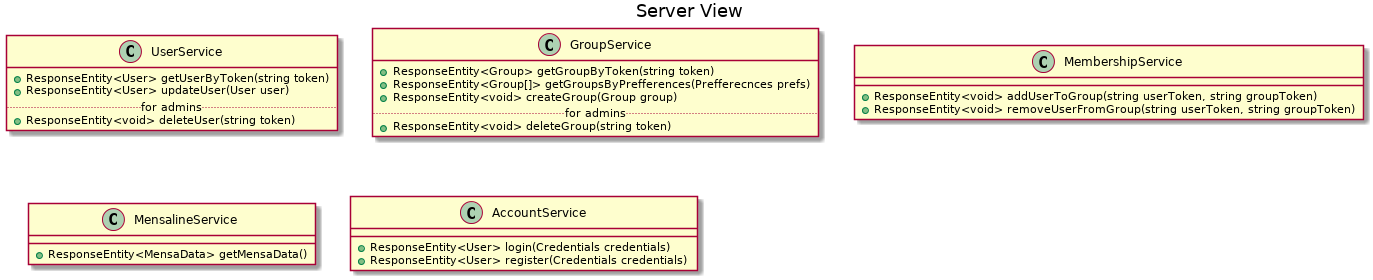
\includegraphics[width=0.93\textwidth]{Klassendiagramme/serverViewCD.png}
\end{center}


\\Alle folgenden Klassen haben keine Konstruktoren, da sie keine Instanzen besitzen sollen,sondern lediglich statische Funktionen beinhalten, die die Schnittstelle des Servers bilden. Da alle Rückgabetypen vom Typ ResponseEntity sind werden auch alle http status codes die auftreten können beschrieben.

\subsubsection{Class UserService}
\subsubsection*{Beschreibung}
Diese Klasse stellt die für den Client benötigten Funktionen bereit um User Daten abzufragen und zu bearbeiten. 

\subsubsection*{Methoden}
\begin{addmargin}[25pt]{0pt}
\begin{itemize}

\item \texttt{ResponseEntity<User> getUserByToken(string token)}\\
	Liefert den User mit dem übergebenen Token. 

	\subsubsection*{Parameter}
	\begin{itemize}
	\item token \\
		Der Token, mit dem der User eindeutig identifizierbar ist.
	\end{itemize}

	\subsubsection*{Rückgabewert}
	Der gesuchte User als ResponseEntity mit status code 200.
	Status code 404, falls der User mit dem Token nicht existiert.

\item \texttt{ResponseEntity<User> updateUser(User user)}\\
	Updated den User auf dem Server mit dem übereinstimmenden Token.

	\subsubsection*{Parameter}
	\begin{itemize}
	\item user \\
		Der User der geupdated werden soll.
	\end{itemize}

	\subsubsection*{Rückgabewert}
	Der geupdatete User als ResponseEntity mit status code 200.
	Status code 404, falls der User mit dem Token nicht existiert.
	
\item \texttt{ResponseEntity<void> deleteUser(string token)}\\
	Löscht den User auf dem Server mit dem übereinstimmenden Token.

	\subsubsection*{Parameter}
	\begin{itemize}
	\item token \\
		Der Token des User, der gelöscht werden soll.
	\end{itemize}

	\subsubsection*{Rückgabewert}
	Status code 200, falls der User gefunden und gelöscht werden konnte.
	Status code 404, falls der User mit dem Token nicht existiert.
	
\end{itemize}
\end{addmargin}

%---------------------

\subsubsection{Class GroupService}
\subsubsection*{Beschreibung}
Diese Klasse stellt die für den Client benötigten Funktionen bereit um Gruppen Daten abzufragen und zu bearbeiten. 

\subsubsection*{Methoden}
\begin{addmargin}[25pt]{0pt}
\begin{itemize}

\item \texttt{ResponseEntity<Group> getGroupByToken(string token)}\\
	Liefert die Gruppe mit dem übergebenen Token. 

	\subsubsection*{Parameter}
	\begin{itemize}
	\item token \\
		Der Token, mit dem die Gruppe eindeutig identifizierbar ist.
	\end{itemize}

	\subsubsection*{Rückgabewert}
	Die gesuchte Gruppe als ResponseEntity mit status code 200.
	Status code 404, falls die Gruppe mit dem Token nicht existiert.

\item \texttt{ResponseEntity<Group[]> getGroupsByPrefferences(Prefferecnces prefs)}\\
	Liefert alle Gruppen, die zu den übergebenen Präferenzen passen.

	\subsubsection*{Parameter}
	\begin{itemize}
	\item prefs \\
		Die Präferenzen, mit denen die Gruppen gesucht werden sollen.
	\end{itemize}

	\subsubsection*{Rückgabewert}
	Ein Array aller passenden Gruppen als ResponseEntity mit status code 200.
	
\item \texttt{ResponseEntity<void> createGroup(Group group)}\\
	Erstellt eine Gruppe auf dem Server.

	\subsubsection*{Parameter}
	\begin{itemize}
	\item group \\
		Die Gruppe, die erstellt werden soll.
	\end{itemize}

	\subsubsection*{Rückgabewert}
	Die erstellte Gruppe mit einen generierten token als ResponseEntity, mit status code 200.
	
\item \texttt{ResponseEntity<void> deleteGroup(string token)}\\
	Löscht die Gruppe auf dem Server mit dem übereinstimmenden Token.

	\subsubsection*{Parameter}
	\begin{itemize}
	\item token \\
		Der Token der Gruppe, die gelöscht werden soll.
	\end{itemize}

	\subsubsection*{Rückgabewert}
	Status code 200, falls die Gruppe gefunden und gelöscht werden konnte.
	Status code 404, falls die Gruppe mit dem Token nicht existiert.


\end{itemize}
\end{addmargin}

%---------------

\subsubsection{Class MembershipService}
\subsubsection*{Beschreibung}
Diese Klasse stellt die für den Client benötigten Funktionen bereit um die Mitgliedschaft von Usern bei Gruppen zu bearbeiten. 

\subsubsection*{Methoden}
\begin{addmargin}[25pt]{0pt}
\begin{itemize}

\item \texttt{ResponseEntity<void> addUserToGroup(string userToken, string groupToken)}\\
	Fügt einen User einer Gruppe bei.

	\subsubsection*{Parameter}
	\begin{itemize}
	\item userToken \\
		Der Token, mit der User eindeutig identifizierbar ist.
	\item groupToken \\
		Der Token, mit dem die Gruppe eindeutig identifizierbar ist.
	\end{itemize}

	\subsubsection*{Rückgabewert}
	Status code 404, falls der User oder die Gruppe nicht gefunden werden konnte.
	Status code 200, sonst.

\item \texttt{ResponseEntity<void> removeUserFromGroup(string userToken, string groupToken)}\\
	Entfernt einen User von einer Gruppe.

	\subsubsection*{Parameter}
	\begin{itemize}
	\item userToken \\
		Der Token, mit der User eindeutig identifizierbar ist.
	\item groupToken \\
		Der Token, mit dem die Gruppe eindeutig identifizierbar ist.
	\end{itemize}

	\subsubsection*{Rückgabewert}
	Status code 404, falls der User oder die Gruppe nicht gefunden werden konnte.
	Status code 200, sonst.
\end{itemize}
\end{addmargin}	

%---------------


\subsubsection{Class MensalineService}
\subsubsection*{Beschreibung}
Diese Klasse stellt die für den Client benötigten Funktionen bereit um die Daten der Mensalinien abzufragen. 

\subsubsection*{Methoden}
\begin{addmargin}[25pt]{0pt}
\begin{itemize}

\item \texttt{ResponseEntity<MensaData> getMensaData()}\\
	Liefert die aktuellen Daten der Mensalinien.

	\subsubsection*{Rückgabewert}
	Die aktuellen Angebote der Mensa.

\end{itemize}
\end{addmargin}
%---------------

\subsubsection{Class AccountService}
\subsubsection*{Beschreibung}
Diese Klasse stellt die für den Client benötigten Funktionen bereit um sich zu registrieren und anzumelden. 

\subsubsection*{Methoden}
\begin{addmargin}[25pt]{0pt}
\begin{itemize}

\item \texttt{ResponseEntity<User> login(Credentials credentials)}\\
	Loggt einen User ein.

	\subsubsection*{Parameter}
	\begin{itemize}
	\item credentials \\
		Die Email-Adresse und das Passwort des Users
	\end{itemize}

	\subsubsection*{Rückgabewert}
	Der User als ResponseEntity mit status code 200.
	Status code 404, die email nicht vorhanden ist.
	Status code 401, falls das Passwort falsch ist.

\item \texttt{ResponseEntity<User> register(Credentials credentials)}\\
	Registriert einen neuen User und generiert ein Token.

	\subsubsection*{Parameter}
	\begin{itemize}
	\item credentials \\
		Die Email-Adresse und das Passwort für den neuen User

	\end{itemize}

	\subsubsection*{Rückgabewert}
	Der neue User, mit dem Token als ResponseEntity mit status code 200.
	Status code 406, die Email-Adresse schon benutzt wird.
	Status code 400, falls die Form der Anfrage falsch ist. Bsw. die Email-Adresse eine falsche Form hat.
		

\end{itemize}
\end{addmargin}

%-------------- Java Doc for the server controller package --------------



\subsection{package.edu.kit.mensameet.controller}
\begin{center}
	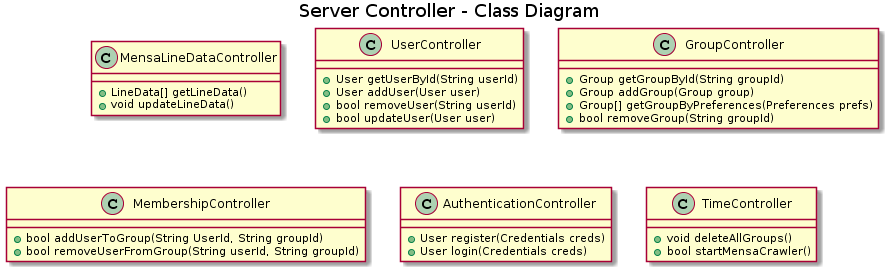
\includegraphics[width=0.93\textwidth]{Klassendiagramme/serverControllerCD.png}
\end{center}
\subsubsection{Class UserController}
\subsubsection*{Beschreibung}
Diese Klasse ist der User Controller und beinhaltet die für den User zuständigen Methoden

\subsubsection*{Methoden}
\begin{addmargin}[25pt]{0pt}
\begin{itemize}

\item public User getUser(String userToken)\\
	Mit dieser Methode wird eine Anfrage nach einem Userprofil gestellt. Es wird nach dem eindeutigen User Token gesucht
	\subsubsection*{Parameter}
	\begin{itemize}
	\item userToken \\
		Eindeutiger Token eines Userprofils
	\end{itemize}
	\subsubsection*{Rückgabewert}
	\begin{itemize}
	\item Userprofil
	\end{itemize}

\item public User addUser(User user)\\
	Diese Methode fügt einen User zur Datenbank hinzu
	\subsubsection*{Parameter}
	\begin{itemize}
	\item user \\
		Eindeutiges Userprofil
	\end{itemize}
	\subsubsection*{Rückgabewert}
	\begin{itemize}
	\item Userprofil
	\end{itemize}
	
\item public bool removeUser(String userToken)\\
	Diese Methode löscht ein Userprofil aus der Datenbank
	\subsubsection*{Parameter}
	\begin{itemize}
	\item userToken \\
		Eindeutiger Token eines Userprofils
	\end{itemize}
	\subsubsection*{Rückgabewert}
	\begin{itemize}
	\item Wird das Userprofil erfolgreich gelöscht, so wird eine Bestätigung zurückgegeben. Wenn der Löschvorgang fehlschlägt wird eine Fehlermeldung zurückgegeben
	\end{itemize}


\item public bool updateUser(User user)\\
	Diese Methode überschreibt ein bestehendes Userprofil mit einem Userprofil des selben Tokens, aber geänderten Parametern
	\subsubsection*{Parameter}
	\begin{itemize}
	\item user \\
		Eindeutiges Userprofil mit geänderten Parametern (bis auf Token)
	\end{itemize}
	\subsubsection*{Rückgabewert}
	\begin{itemize}
	\item Wird das Userprofil erfolgreich überschrieben, so wird eine Bestätigung zurückgegeben. Wenn das Überschreiben fehlschlägt wird eine Fehlermeldung zurückgegeben
	\end{itemize}
\end{itemize}

\end{addmargin}

\subsubsection{Class GroupController}
\subsubsection*{Beschreibung}
Diese Klasse ist der Group Controller und beinhaltet die für die Gruppen zuständigen Methoden

\subsubsection*{Methoden}
\begin{addmargin}[25pt]{0pt}
\begin{itemize}

\item public Group getGroup(String groupToken)\\
	Mit dieser Methode wird eine Anfrage nach einer Gruppe gestellt. Es wird nach dem eindeutigen Group Token gesucht
	\subsubsection*{Parameter}
	\begin{itemize}
	\item groupToken \\
		Eindeutiger Gruppen Token
	\end{itemize}
	\subsubsection*{Rückgabewert}
	\begin{itemize}
	\item Gruppe 
	\end{itemize}
	
\item public Group addGroup(Group group)\\
	Diese Methode fügt eine Gruppe zur Datenbank hinzu
	\subsubsection*{Parameter}
	\begin{itemize}
	\item group \\
		Gruppe mit korrekten Parametern
	\end{itemize}
	\subsubsection*{Rückgabewert}
	\begin{itemize}
	\item Die hinzugefügte Gruppe wird zurückgegeben
	\end{itemize}
	
\item public Group[] getGroupByPreferences(Preferences prefs)\\
	Diese Methode sucht nach Gruppen mit den passenden Präferenzen
	\subsubsection*{Parameter}
	\begin{itemize}
	\item prefs \\
		Nötige Präferenzen zur Findung einer passenden Gruppe (Linie und Uhrzeit)
	\end{itemize}
	\subsubsection*{Rückgabewert}
	\begin{itemize}
	\item Es werden alle Gruppen mit übereinstimmenden Präferenzen zurückgegeben
	\end{itemize}

\item public bool removeGroup(String groupToken)\\
	Diese Methode löscht eine Gruppe aus der Datenbank
	\subsubsection*{Parameter}
	\begin{itemize}
	\item groupToken \\
		Eindeutiger Group Token der zu löschenden Gruppe
	\end{itemize}
	\subsubsection*{Rückgabewert}
	\begin{itemize}
	\item Wird die Gruppe erfolgreich gelöscht, so wird eine Bestätigung zurückgegeben. Wenn der Löschvorgang fehlschlägt wird eine Fehlermeldung zurückgegeben
	\end{itemize}
\end{itemize}
\end{addmargin}

\subsubsection{Class MensaDataController}
\subsubsection*{Beschreibung}
Diese Klasse ist der Mensadaten Controller und enthält die Methoden, die für die Verwaltung der Mensadaten zuständig sind

\subsubsection*{Methoden}
\begin{addmargin}[25pt]{0pt}
\begin{itemize}

\item public LineData[] getLineData()\\
	Diese Methode fragt die Datenbank nach dem tagesaktuellen Speiseplan ab

	\subsubsection*{Rückgabewert}
	\begin{itemize}
	\item Es werden alle Essenslinien mit tagesaktuellem Menü zurückgegeben
	\end{itemize}
	
\item public void updateLineData()\\
	Diese Methode beinhaltet einen Crawler der den tagesaktuellen Speiseplan der Mensa vom Studentenwerk bezieht und anschließend in der Datenbank speichert
\end{itemize}
\end{addmargin}

\subsubsection{Class MembershipController}
\subsubsection*{Beschreibung}
Diese Klasse ist der Membership Controller und beinhaltet die Methoden, die für die Gruppenmitgliedschaft der einzelnen User zuständig sind

\subsubsection*{Methoden}
\begin{addmargin}[25pt]{0pt}
\begin{itemize}

\item public bool addUserToGroup(String UserToken, String groupToken)\\
	Diese Methode fügt einen User zu einer Gruppe hinzu
	\subsubsection*{Parameter}
	\begin{itemize}
	\item userToken \\
		Eindeutiger Token des Users der zur Gruppe hinzugefügt werden soll
	\item groupToken \\
		Eindeutiger Token der Gruppe, zu der der User hinzugefügt werden soll
	\end{itemize}
	\subsubsection*{Rückgabewert}
	\begin{itemize}
	\item Falls das Hinzufügen zur Gruppe erfolgreich war, wird eine Bestätigung zurückgegeben. Eine Fehlermeldung falls nicht.
	\end{itemize}
	
\item public bool removeUserFromGroup(String userToken, String groupToken)\\
	Diese Methode entfernt einen User aus einer Gruppe
	\subsubsection*{Parameter}
	\begin{itemize}
	\item userToken \\
		Eindeutiger Token des Users, der aus der Gruppe entfernt werden soll
	\item groupToken \\
		Eindeutiger Token der Gruppe, aus der der User entfernt werden soll
	\end{itemize}
	\subsubsection*{Rückgabewert}
	\begin{itemize}
	\item Falls das Entfernen aus der Gruppe erfolgreich war, wird eine Bestätigung zurückgegeben. Eine Fehlermeldung falls nicht.
	\end{itemize}
\end{itemize}
\end{addmargin}

\subsubsection{Class AuthenticationController}
\subsubsection*{Beschreibung}
Diese Klasse ist der Authentication Controller und beinhaltet die Methoden, die für die Registrierung und das Anmelden eines Users zuständig sind

\subsubsection*{Methoden}
\begin{addmargin}[25pt]{0pt}
\begin{itemize}

\item public User register(Credentials creds)\\
	Diese Methode ist für die Registrierung eines Users zuständig
	\subsubsection*{Parameter}
	\begin{itemize}
	\item creds \\
		Die vom User festgelegten Daten zur Registrierung, bestehend aus E-Mail und Passwort
	\end{itemize}
	\subsubsection*{Rückgabewert}
	\begin{itemize}
	\item Es wird ein leeres Userprofil zurückgegeben
	\end{itemize}
	
\item public User login(Credentials creds)\\
	Diese Methode ist für die Ameldung eines Users zuständig
	\subsubsection*{Parameter}
	\begin{itemize}
	\item creds \\
		Die vom User bei der Registrierung festgelegten Daten, bestehend aus E-Mail und Passwort
	\end{itemize}
	\subsubsection*{Rückgabewert}
	\begin{itemize}
	\item Es wird das UserProfil des Users zurückgegeben
	\end{itemize}

\end{itemize}
\end{addmargin}

\subsubsection{Class TimeController}
\subsubsection*{Beschreibung}
Diese Klasse ist der Time Controller und beinhaltet die Methoden, die für die zeitlich festgelegte Abläufe zuständig ist

\subsubsection*{Methoden}
\begin{addmargin}[25pt]{0pt}
\begin{itemize}

\item public void deleteAllGroups()\\
	Diese Methode löscht am Ende des Tages alle Gruppen
	
\item public bool startMensaCrawler()\\
	Diese Methode startet jeden Morgen den Aufruf zum Abrufen der Mensadaten
	\subsubsection*{Rückgabewert}
	\begin{itemize}
	\item Wurden die Mensadaten erfolgreich abgegriffen, wird eine Bestätigung zurückgegeben. Eine Fehlermeldung falls nicht.
	\end{itemize}

\end{itemize}
\end{addmargin}


\section{HTTP Protokoll}

Die REST Endpoints die in der Tabelle aufgelistet sind werden für die Kommunikation zwischen Client und Server verwendet. \\

\resizebox{16cm}{!} {
\begin{tabu} { | l | l | l | l | } 
 \hline
 Request Type & Endpoint & Payload & Beschreibung \\ [0.5ex] 
 \hline
 GET  & /user/\{token\} &  & Liefert den User mit dem übergebenem Token. \\ 
 
 POST & /user  & User & Updated den User (Token liegt in User) \\ 
 \hline
GET & /group/{token} & & Liefert die Gruppe mit dem übergebenem Token. \\
POST & /group-prefferences & Preferrences & Liefert alle Gruppen die zu den übergebenen Prefferenzen passen. \\
POST  & /create-group/  & Group & Erstellt die übergebene Gruppe. \\
DELETE  & /group/\{token\} & & Löscht die Gruppe mit dem übergebenen Token. \\

\hline 

POST  & /add-user-to-group?user=\{userToken\}\&group={groupToken} & & Fügt den User mit dem userToken zu der Gruppe mit dem groupToken. \\
POST  & /remove-user-from-group?user=\{userToken\}\&group={groupToken} & & Entfernt den User mit dem userToken von der Gruppe mit dem groupToken. \\

\hline

POST & /login & email, password & Meldet den Client an dem Account mit den übergebenen Anmeldedaten an. \\
POST & /register & email, password & Erstellt einen Account mit den übergebenen Anmeldedaten. \\

\hline

GET &  /mensadata & & Liefert die aktuellen Mensadaten.\\

\hline

\end{tabu}
}




\chapter{Datenstrukturen}

\begin{center}
	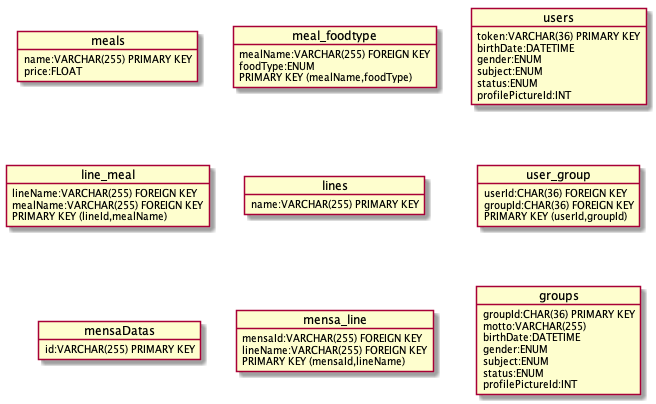
\includegraphics[width=0.93\textwidth]{Objektdiagramme/datenstrukturen.png}
\end{center}
In der Abbildung sieht man die Datenstruktur der Datenbank, also die Tabellen, die es in der Datenbank geben wird. Weil wir mySQL verwenden und mySQL nicht List-Type als Datentype unterstützt, speichern wir Liste in Form von extra Tabellen.

\chapter{Dynamische Modelle}
\section{Aktivitätsdiagramm}

\section{Sequenzdiagramm}
\subsection{Registrieren}
\begin{center}
	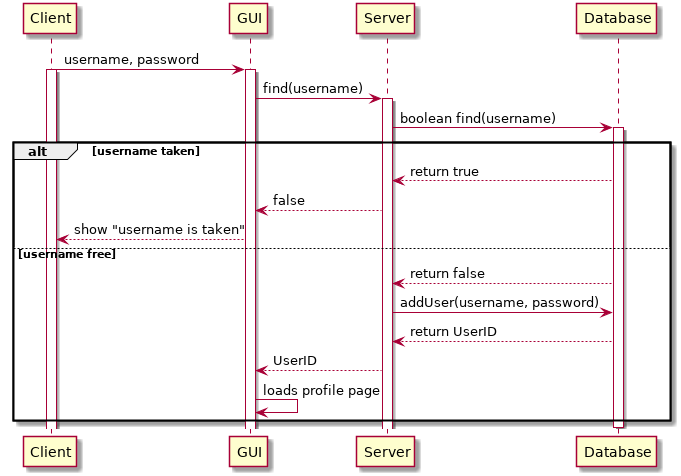
\includegraphics[width=0.93\textwidth]{Sequenzdiagramme/Registration.png}
\end{center}
\subsection*{Beschreibung}
Bob öffnet zum ersten mal die Applikation MensaMeet und sieht den Registrierungsbildschrim. Dort soll er seine E-Mailadresse und ein Passwort eingeben. Sobald er das getan hat, werden die Daten an der Server geschickt, welcher sie an Firebase weiterleitet. Firebase legt auf seinem Server den User an und generiert ein Token zur UserIdentifikation. Das Token wird an den Server zurückgegeben, der damit einen User in der Datenbank anlegt und das Userobjekt an den Client schickt. Auf dem Client (Bobs Smartphone) wird der User/Token gespeichert und bei jeder zukünftigen Anfrage an den Server mitgegeben. 
Bob sieht nun den Bildschirm zur Profilbearbeitung. Die Eingabe der Profildaten ist Pflicht, vorher kann er nicht weiter zu einer anderen Seite gelangen.
Nachdem er seinen Nutzernamen, Motto, Alter, Geschlecht, Status, Fachrichtung eingegeben hat, werden diese Daten an den Server gesendet, der damit das Userprofil in der Datenbank aktualisiert. 
\newpage
\subsection{Mensalinien wählen}
\begin{center}
	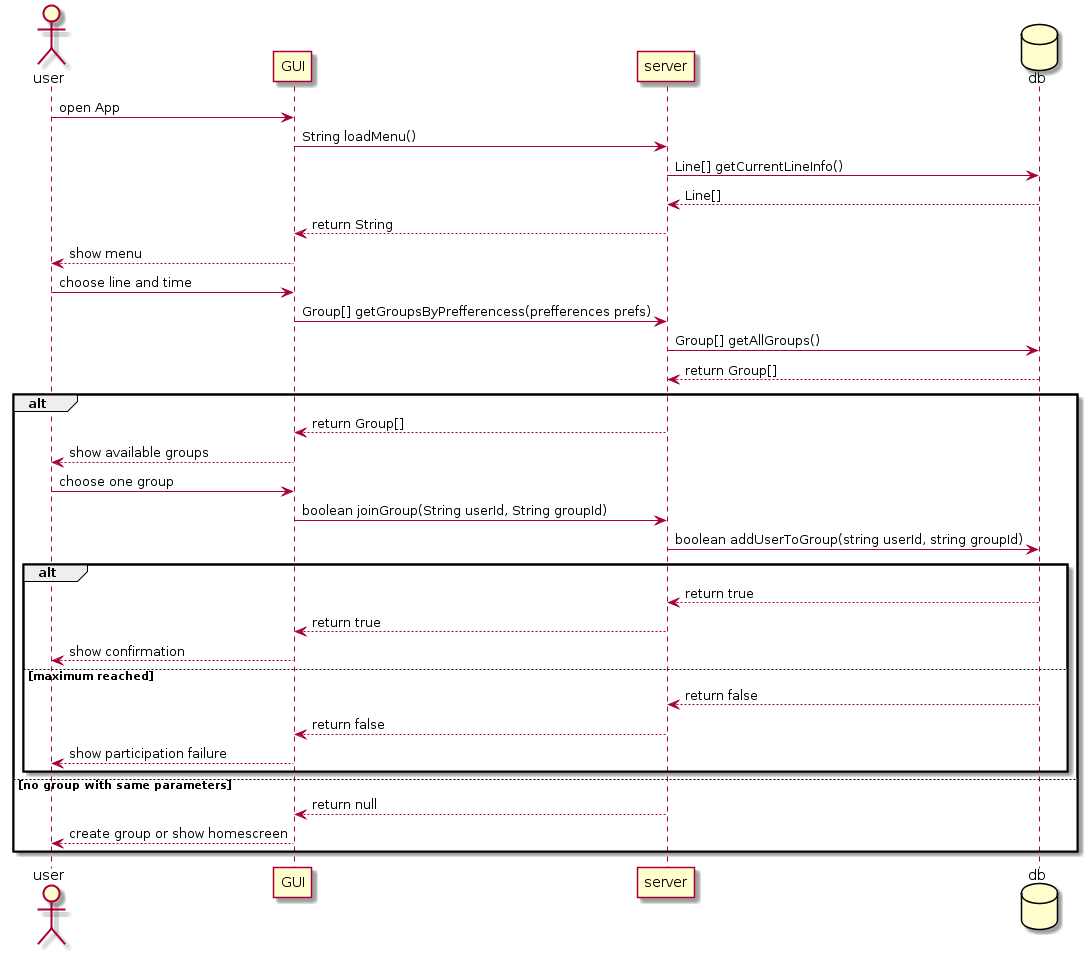
\includegraphics[width=0.93\textwidth]{Sequenzdiagramme/chooseLineAndTimeSD.png}
\end{center}
\subsection*{Beschreibung}
Der Nutzer öffnet die Anwendung (die Registrierung ist bereits erfolgt). Nun soll er als Scrolldown-menü die Mensalinien mit ihrem jeweiligen Angebot zu sehen kriegen (Dies ist der "HomeScreen"). Dazu werden die Mensadaten über den Server von der Datenbank angefragt, aufbereitet und dem Client übermittelt. Dieser kann nun die Linien anklicken an denen er gern essen möchte. Danach stellt er das für ihn geeignete Zeitintervall ein. Diese Daten werden dem Server übermittelt, welcher sich die Gruppen aus der Datenbank holt, nach den angegebenen Daten filtert und an den Client übergibt. Der Nutzer kann sich die Gruppen anschauen und einer davon beitreten. Beim Versuch beizutreten wird dem Server der User- und der GroupToken übermittelt. Es wird überprüft ob die Gruppe bereits voll ist, ist dies der Fall, erhält der Client eine Fehlermeldung und gelangt wieder zur Gruppenübersicht. Ist noch Platz in der Gruppe, wird die Gruppe in der Datenbank aktualisiert, indem der User hinzugefügt wird. Dann wird über den Server eine Bestätigung an den Client geschickt und der Nutzer gelangt zur Gruppenseite. 
Falls keine Gruppen passend zu den Angaben des Clients gefunden wurde, erhält der Client eine passende Fehlermeldung und kann entweder zurück zum HomeScreen oder selbst eine Gruppe erstellen.

\newpage
\subsection{Gruppe beitreten}
\begin{center}
	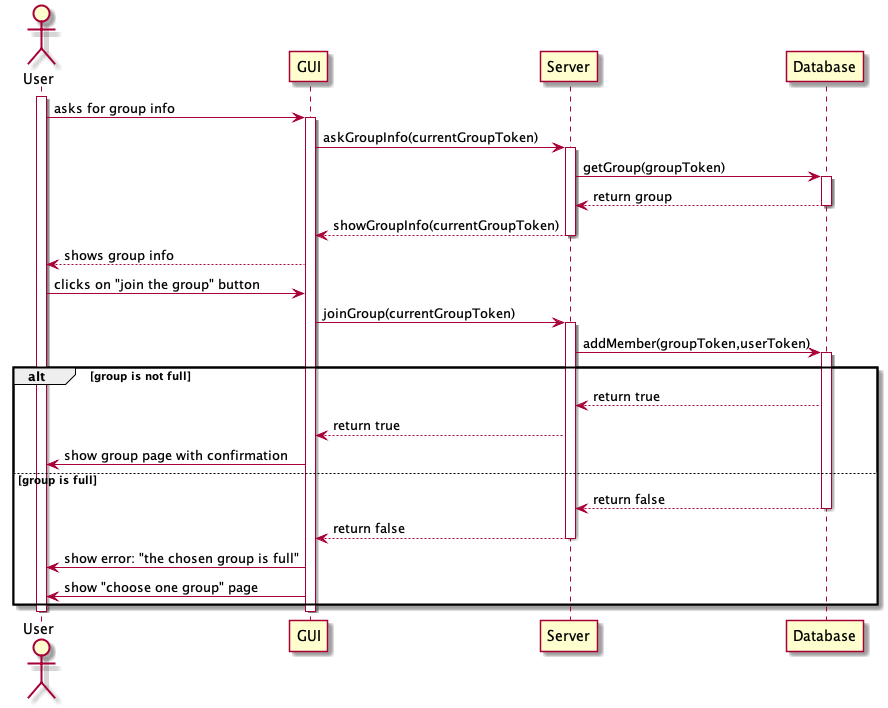
\includegraphics[width=0.93\textwidth]{Sequenzdiagramme/checkInfoAndJoinGroupSD.png}
\end{center}


\subsection*{Beschreibung}
Nachdem der Nutzer, passend zu seinen ausgewählten Linien und seinem eingestellten Zeitintervall, Gruppen in einem Scrolldown-menü angezeigt bekam, klickt er nun eine Gruppe an, um mehr Informationen zu ihr zu sehen. Dazu wird an den Server eine Anfrage mit dem GroupToken gesendet. Der Server sucht damit nach der Gruppe in der Datenbank und übermittelt die Informationen dem Client. Beim User wird die angeklickte Gruppe nach unten aufgklappt, so dass nun zusätzlich zur Linie, Startzeit und Motto auch die Mitgliederliste und den "Beitreten"-Button sieht. Er drückt auf "Beitreten". Nun wird dem Server die UserID und GroupID übermittelt. Er prüft in der Datenbank ob die Gruppe inzwischen voll ist. Ist dies der Fall, erhält der Client eine Fehlermeldung : "Deine gewählte Gruppe ist bereits voll" und gelangt wieder zur Gruppenübersicht. Ist noch Platz in der Gruppe, wird die Datenbank aktualisiert und dem Client der Beitritt bestätigt. Der Nutzer gelangt zur Detailansicht seiner Gruppe. Er steht nun ebenfalls in der Mitgliederliste und sieht den Button "Gruppe Verlassen".

\newpage
\subsection{Gruppe erstellen}
\begin{center}
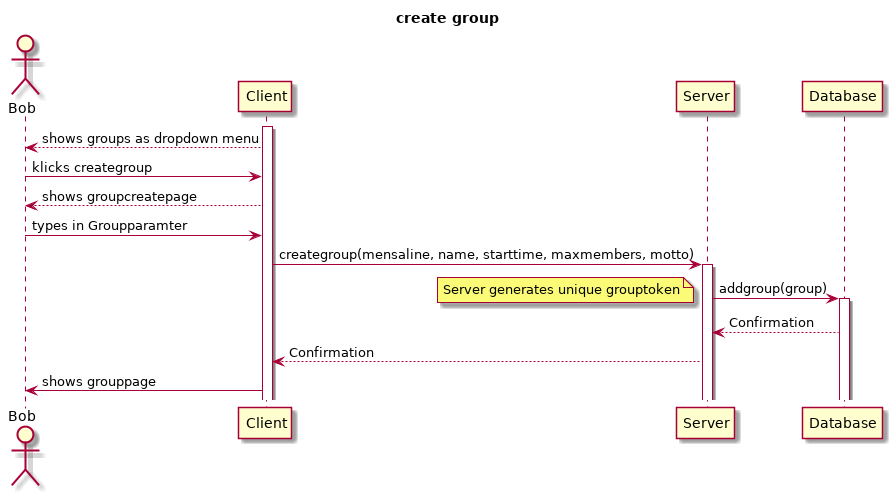
\includegraphics[width=0.93\textwidth]{Sequenzdiagramme/CreateGroup.png}

\end{center}
\subsection*{Beschreibung}
Nachdem der User die zu ihm passenden Gruppen angefragt hat, aber keine gefunden wurde entscheidet er sich eine Gruppe zu erstellen. Er stellt dazu die erforderlichen Gruppenparameter(Gruppenname, Mensalinie, Startzeit, Motto, Maximale Mitgliederzahl) ein. Der Server erhält die Anfrage mit diesen Paramtern eine neue Gruppe anzulegen. Er generiert (aus dem Namen?) ein eindeutiges groupToken und legt die Gruppe in der Datenbank an. Dem Client wird die erfolgreiche Gruppengründung bestätigt und ihm wird als nächstes die Detailansicht seiner Gruppe angezeigt.

\newpage
\subsection{Gruppe verlassen}
\begin{center}
	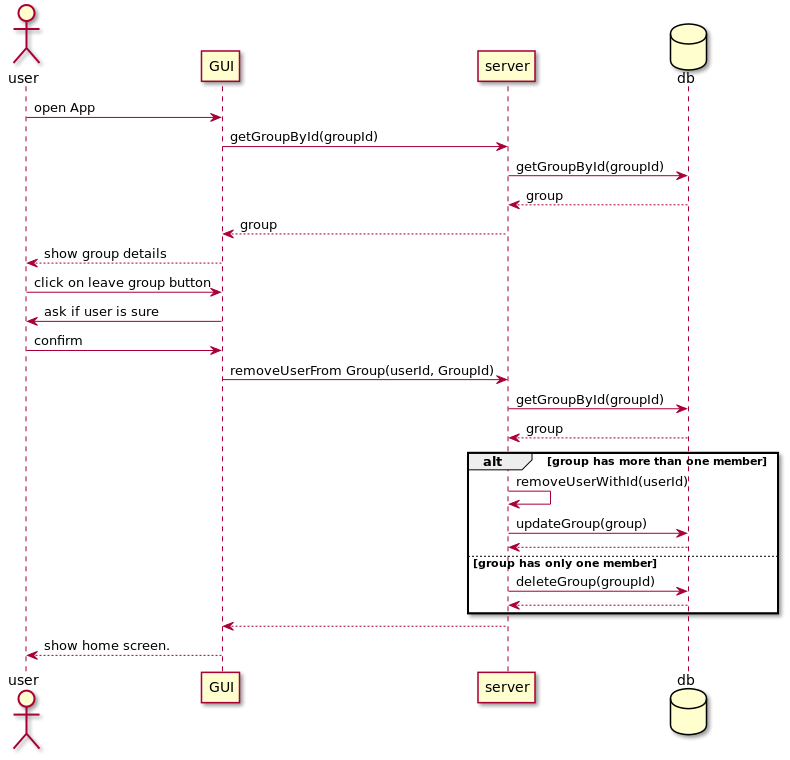
\includegraphics[width=0.93\textwidth]{Sequenzdiagramme/leaveGroupSD.png}
\end{center}

\subsection*{Beschreiung}
Der Nutzer öffnet die App MensaMeet. Da er bereits Mitglied einer Gruppe ist, wird ihm die Detailansicht seiner Gruppe angezeigt.
In dieser Ansicht ist ein Button "Gruppe verlassen". Er drückt diesen Button und muss seine Entscheidung bestätigen. Für den Austritt wird dem Server der User- und GroupToken übermittelt. Der Server sucht anhand des GroupToken die Gruppe in der Datenbank um sie zu aktualisieren. Der User wird aus der Gruppe entfernt und die Mitgliederzahl der Gruppe überprüft. Ist diese nun bei 0, so wird die Gruppe aus der Datenbank gelöscht.
Der Client erhält in jedem Fall die Bestätigung zum Austritt aus der Gruppe und wird wieder zum HomeScreen überführt.


\chapter{Änderungen zum Pflichtenheft}
\begin{itemize}
	\item Nutzername und Gruppennamen müssen nicht mehr eindeutig sein \\
	stattdessen wird für den Nutzer von Firebase ein eindeutiges Token generiert, das als Identifikator dient. Für Gruppen wird ebenfalls ein eindeutiges Token durch den Server generiert.
	\item Zum Registrieren wird statt Nutzername und Password nun Email und Passwort benötigt. \\Diese Änderung ist bedingt durch die Nutzung von Firebase und erfüllt damit eines unserer Wunschkriterien: Dass eine Email Verifikation beim Registrieren stattfindet. 
\end{itemize}

\chapter{Glossar}

\chapter{Anhang}

\end{document}
